
\documentclass[preview,border=0.80001bp, convert=imagemagick]{standalone}
%\documentclass{article}
\usepackage{hyperref}
\usepackage{amsmath}
\usepackage{tikz}
\usepackage{miama}
\usepackage{xcolor}
\usepackage[T1]{fontenc}

\usepackage{pgfplots}

\newlength\unitlen
\tikzset{
    unit length/.code={\setlength{\unitlen}{#1}},
    unit length = 8pt
}

\begin{document}
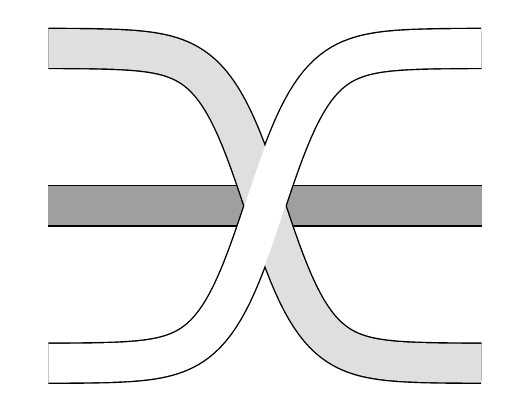
\begin{tikzpicture}
    \def\mm{14}
    \def\M{15}
    \def\N{100}
    \def\xa{-2.75}
    \def\xb{2.75}
    %\def\ya{-2.5}
    %\def\yb{2.5}
    %\draw (2.5,0) node[circle, minimum size = \M pt,inner sep = 0pt, outer
    %sep = 0pt,fill=black] {};
    %\draw (-2.5,0) node[circle, minimum size = \M pt,inner sep = 0pt, outer
    %sep = 0pt,fill=black] {};

    %\draw (2.5,1.999) node[circle, minimum size = \M pt,inner sep = 0pt, outer
    %sep = 0pt,fill=black] {};
    %\draw (-2.5,1.999) node[circle, minimum size = \M pt,inner sep = 0pt, outer
    %sep = 0pt,fill=black] {};
    %\draw (2.5,-1.999) node[circle, minimum size = \M pt,inner sep = 0pt, outer
    %sep = 0pt,fill=black] {};
    %\draw (-2.5,-1.999) node[circle, minimum size = \M pt,inner sep = 0pt, outer
    %sep = 0pt,fill=black] {};

    \draw[color=black, line width = \M pt] (\xa,0) -- (\xb,0);
    \draw[color=gray!75, line width = \mm pt] (\xa,0) -- (\xb,0);

    \draw[color=black,samples=\N,domain=\xa:\xb, line width = \M pt] % SIN
    plot(\x,{2 * (1 - exp(-\x*3))/ (1 + exp(-\x*3))}) % r for radians
    %%node[above right] at (5*pi/2,1) {$\sin(x)$};
    ;
    \draw[color=black,samples=\N,domain=\xa:\xb, line width = \M pt] % SIN
    plot(\x,{-2 * (1 - exp(-\x*3))/ (1 + exp(-\x*3))}) % r for radians
    %%node[above right] at (5*pi/2,1) {$\sin(x)$};
    ;
    \draw[color=gray!25,samples=\N,domain=\xa:\xb,line width = \mm pt] % SIN
    plot(\x,{-2 * (1 - exp(-\x*3))/ (1 + exp(-\x*3))}) % r for radians
    %%node[above right] at (5*pi/2,1) {$\sin(x)$};
    ;
    \draw[color=white,samples=\N,domain=\xa:\xb, line width= \mm pt] % SIN
    plot(\x,{2 * (1 - exp(-\x*3))/ (1 + exp(-\x*3))}) % r for radians
    %%node[above right] at (5*pi/2,1) {$\sin(x)$};
    ;

\end{tikzpicture}
\end{document}
